\section{Technologies used}

This section presents an overview of the key technologies used and their place in the PaWS framework: Tpips, Python, Pylons, Virtual Environment and Web application technologies (Javascript, Ajax and JQuery)

\subsection{Tpips}
\label{tpips_interface}
\emph{Tpips} is the line interface and scripting language of the PIPS project. It allows to use all of the PIPS functionalities in easier (more user-friendly) way, because it simplifies usage of database when performing operations, it handles all accesses to database, for instance itself.
Due to using PIPS metavariables (like \%ALL) Tpips enables application of PIPS command to several modules with one command. Another advantage of this interface is the fact that it provides on-line help (list of commands and automatic completion).
Tpips is a great tool for all tasks which are repeatable and do not require any interaction with the user.

In the PAWS project the Tpips interface is used to perform demo. On source file, even if it was modified by user, there is Tpips script performed with prepared, always the same set of well-known operations. That allows to separate the indivudual steps and their results which are shown to user one by one. Also Tpips script may be more understandable for new user than PYPS code.

\subsection{Python}
\label{python_description}
Python is a portable\footnote{It runs on Windows, Linux/Unix, Mac OS and has been ported to the Java and .NET virtual machines}, script programming language. Python is one of the most commonly used procedural programming languages because of clearness of its syntax, intuitive object orientation, extensibility provided by modularity - modules can be written not only in Python but even in C or Java and very high level dynamic data types. One of the major advantages of Python language is its ability of being used by applications as a scripting interface.
There is also a lot of tools based on this language. They are easy to integrate and to extend. It was the main advantage of using Pylons Project\cite{pylons} - web application framework technology based on Python. Due to that, PyPS (PIPS Python interface) could be easily linked to web technologies was simplified.

\begin{figure}[h!]
  \centering
  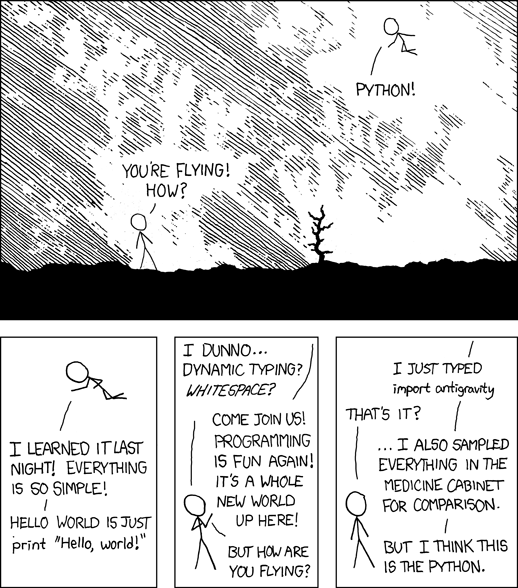
\includegraphics[width=0.6\textwidth]{reportCh2/python}
  \caption{Python by xkcd\cite{python_xkcd}}
  \label{fig:python}
\end{figure}

\subsection{Virtual Environment}
\label{virtualenv}
Virtualenv\cite{virtualenvlit} is the tool used to create isolated Python environments. Thanks to that, it is possible to make several distinct environments, which share the same version of Python, but can have different sets of modules, libraries and packages. All of them are installed in the Python \emph{site-packages} directory.

This tool is protecting applications against conflicts caused by different requirements.

\subsection{Pylons}
\label{pylons_descriptions}
Pylons \cite{pylons} is an flexible Python framework based on the MVC\footnote{MVC stands for \emph{Model-View-Controller}, more in section \ref{mvc}} design pattern and WSGI\footnote{WSGI\cite{wsgi} stands for \emph{Web Server Gateway Interface} and it is the Python standard which specifies interface between web servers and web applications.} standard. Besides base web application server functions, Pylons provides also a set of tools and libraries which extend its way of working, but it does not impose the specific solutions and tools should be used. User can decide which modules he/she wants to include in his/her application. This approach assures user that his/her application consists only of necessary modules and it is as light as possible. If it is necessary, adding third-party libraries is also very easy and intuitive. This possibility of choosing, adding and composing modules makes Pylons very flexible and light framework. It is also very easy to learn and to use by new users.

As it is written above, Pylons provides a lot of tools which simplify creating a web application. One of main ones, Routes\cite{routes} framework generates and maps URL addresses to code. Another tool, WebHelpers\cite{webhelpers} is a set of utility functions for generating JavaScript\cite{javascript} code. To create HTML code combined with Python and to pass variables to them, Pylons is using a \emph{templating system}. It allows user to write HTML and embed Python code when it is needed\cite{templating_system}. This solution also supports reusability of the code. The default templating language is Mako\cite{mako}. 

Pylons also can operate on databases (using \emph{Object Relational Managers} like in example SQLAlchemy\cite{sqlalchemy} or SQLObject\cite{sqlobject}). In addition it provides caching mechanisms and manages session variables.

\subsection{Web Application Technologies}
\label{web_application_technologies}

Interactions between users and server are handled by Ajax\cite{ajax} (Asynchronous JavaScript and XML). Due to that technology user view can be refreshed without reloading whole document. It is performed in a asynchronous way, which enables user to execute other operations at the same time. Ajax technology is built in Pylons. 


Ajax is used also by JQuery\cite{jquery}, a light and fast library that contains tools to use Javascript in more advanced way like animations or dynamic modifications of site content. What is important, changes provided by JQuery do not require modifications of HTML code of the site.

\subsection{Other tools}
\label{other_technologies}

\begin{itemize}
  \item {\bf Pygments}\cite{pygments} is a Python syntax highlighting library. It supports a significant number of languages and markup formats. There is also mechanism which allows user to define his/her own parser to recognize user specific language. Pygments can be used as a library or as a command-line tool.
  \item {\bf Pyrops} is a Python module based on {\bf pyro} - PYthon Remote Objects\cite{pyro}. Pyrops was created as a solution for the problem of concurrent accesses to Pips workspaces - it was not possible to work on several workspaces at the same time in a script\cite{pyps_doc}. Pyrops encapsulate each workspace in a new, separate program in a transparent way\footnote{Transparency is provided by RPC (and by pyro)\cite{pyps_pass_manager}}. Usage of Pyrops is easy for Pyps user - Pyrops workspace inherites of Pyps workspace and they are used in the same way.
  \item {\bf GCC}\cite{gcc} - the GNU Compiler Collection is the one of the most popular compiler for C and C++ languages. In PaWS, GCC is used for checking correctness of the user input before performing operations.
  \item {\bf F77}\cite{fortran77} and {\bf gFortran}\cite{gfortran} are Fortran compilers, which compiles Fortran code to C code. They are used in PaWS for the same reason as GCC - to check input source code.
  \item {\bf Fabric}\cite{fabric} - the Python library for automatic deployment and setting up of the application. It can be used as library but also as command-line tool. Creator of the application must provide requirements file where all of the dependencies of the application and its versions are described. A second file must be supplied. It is so called \emph{fabfile.py}. It specifies all the operations (like setup, installation, clean etc.) that can be used.
%%  \item {\bf versioning}
%%   ??
\end{itemize}



